\documentclass{beamer}

\mode<presentation>
{
  \usetheme{Frankfurt}
  \usecolortheme{orchid}
  \setbeamercovered{invisible}
  \setbeamertemplate{footline}[frame number]
}

\usepackage[english]{babel}
\usepackage[latin1]{inputenc}
\usepackage{times}
\usepackage[T1]{fontenc}
\usepackage{tikz}
\usepackage{array}
\usepackage{cancel}


\usetikzlibrary{shapes,backgrounds}

\def\multiset#1#2{\ensuremath{\left(\kern-.3em\left(\genfrac{}{}{0pt}{}{#1}{#2}\right)\kern-.3em\right)}}

\def\blue{\color{blue}~}
\def\black{\color{black}~}
\def\bl[#1]#2{\begin{block}{#1}#2\end{block}}
\def\integers{\mathbb{Z}}
\def\enumb{\begin{enumerate}}
\def\enume{\end{enumerate}}
\def\itemb{\begin{itemize}}
\def\iteme{\end{itemize}}


\usepackage{remreset}
\makeatletter
\@removefromreset{subsection}{section}
\makeatother
\setcounter{subsection}{1}

\title{Discrete Mathematics, Section 001, Fall 2016}
\subtitle{Lecture 15: Counting Functions, Pigeonhole principle}

\author[Zsolt]{Zsolt Pajor-Gyulai \\ \texttt{zsolt@cims.nyu.edu}}
\date{November 2, 2016}

\pgfdeclareimage[height=1cm]{NYUlogo}{NYUlogo.jpg}

\institute[NYU] 
{
\normalsize Courant Institute of Mathematical Sciences
}
\titlegraphic{\pgfuseimage{NYUlogo}}

\begin{document}

\begin{frame}
  \titlepage
\end{frame}

\AtBeginSection[]
{
\begin{frame}
\frametitle{Outline}
\tableofcontents[currentsection]
\end{frame}}

\section{Counting functions}

\begin{frame}{Number of functions between finite sets}
\bl[]{\textbf{Q}: Let $A$ and $B$ be finite sets. How many functions from $A$ to $B$ are there?}
\[
A=\{1,2,\dots,a\},\qquad B=\{1,2,\dots,b\}
\]
\itemb
\item We can write every function as
\[
f=\{(1,?),(2,?),(3,?),\dots,(a,?)\}
\]
where the $?$s are entries from $B$.
\item There are $b$ choices for each $?$.
\iteme
\bl[Proposition]{Let $A$ and $B$ be finite sets with $|A|=a$ and $|B|=b$. The number of functions from $A$ to $B$ is $b^a$.}
\end{frame}

\begin{frame}
If $A=\{1,2,3\}$ and $B=\{4,5\}$ then all the functions $f:A\to B$:
\[
\begin{array}{cc}
\{(1,4),(2,4),(3,4)\}&\{(1,5),(2,4),(3,4)\}\\
\{(1,4),(2,4),(3,5)\}&\{(1,5),(2,4),(3,5)\}\\
\{(1,4),(2,5),(3,4)\}&\{(1,5),(2,5),(3,4)\}\\
\{(1,4),(2,5),(3,5)\}&\{(1,5),(2,5),(3,5)\}
\end{array}
\]
As predicted, there are $2^3=8$ functions.
\bl[Notation]{
The set of all functions from $A$ to $B$ is denoted by $B^A$.
}
Just as it was the case with $2^A$ (all subsets of $A$), this is just a notation which is convenient because then
\[
|B^A|=|B|^{|A|}
\]
\center Do Problem 1 on the worksheet.

\end{frame}

\begin{frame}
\bl[]{\textbf{Q}: Let $A$ and $B$ be finite sets with $|A|=a$ and $|B|=b$.
\itemb
\item How many functions $f:A\to B$ are one-to-one? 
\item How many are onto?
\iteme}
\itemb
\item Let $|A|>|B|$, and assume $f$ is one-to-one. Without loss of generality assume
\[
A=\{1,2,\dots,|A|\},\qquad B=\{1,2,\dots,|B|\}
\]\vspace{-0.4cm}
\itemb
\item Assume that we find what gets mapped to $\{1,2,\dots,|B|\}$.
\item We still have $|A|-|B|$ elements in $A$ to map somewhere, but we ran out of distinct elements in $B$!
\iteme
Therefore $f$ cannot be one-to-one.
\item Let $|A|<|B|$, and assume $f$ is onto.
\itemb
\item Assume that we map all elements in $A$ to an element in $B$. 
\item We still have $|B|-|A|$ elements in $B$ that we haven't covered yet!
\iteme
Therefore $f$ cannot be onto.
\iteme
\end{frame}

\begin{frame}{The pigeonhole principle}

\bl[Proposition (The pigeonhole principle)]{Let $A$ and $B$ be finite sets and let $f:A\to B$. If $|A|>|B|$, then $f$ is not one-to-one. If $|A|<|B|$, then $f$ is not onto.}
The contrapositive of this statement is
\bl[Proposition]{Let $A$ and $B$ be finite sets and let $f:A\to B$. If $f$ is a bijection, then $|A|=|B|$.}
\textbf{Fun fact:} For infinite sets, this becomes the definition of the cardinalities being equal:
\itemb
\item $|\mathbb{N}|=|\mathbb{Z}|$ (later today)
\item $|\mathbb{R}|\neq |\mathbb{Z}|$.
\iteme
\end{frame}

\begin{frame}
\bl[]{\textbf{Q}: Let $A$ and $B$ be finite sets with $|A|=a$ and $|B|=b$.
\itemb
\item How many functions $f:A\to B$ are one-to-one? 
\item How many are onto?
\iteme}\vspace{-0.3cm}
\[
(1,?),(2,?),\dots, (a,?)
\]\vspace{-0.3cm}
\itemb
\item One-to-one when $|A|\leq|B|$:

The $?$-s have to be filled with elements from $B$ without repetition. Therefore
\[
\#\textrm{One-to-one functions}=(b)_{a}=\frac{b!}{(b-a)!}
\]
\item Onto when $|A|\geq|B|$:
The $?$-s have to be filled with elements from $B$ with every element used at least once.
\[
\#\textrm{Onto functions}=\sum_{j=0}^{b}(-1)^j\binom{b}{j}(b-j)^{a}.\qquad (WS2)
\]
\iteme

\end{frame}

\section{Applications of the pigeonhole principle}

\begin{frame}
\bl[Proposition]{Let $n\in\mathbb{N}$. Then there exist positive integers $a$ and $b$, with $a\neq b$, $a,b\leq 11$, such that $n^a-n^b$ is divisible by $10$.}

E.g. $n=17$, then
\[
17^6-17^2=24,137,569-289=24,137,280
\]
\begin{proof}
Consider the $11$ natural number
\[
n^1\qquad n^2\qquad n^3\qquad \dots n^{11}
\]
The last digits of these numbers takes values in $\{0,1,2,\dots,9\}$. Since there are $10$ possible digits and $11$ different numbers, two of these numbers, let's say, $n^a,n^b$, will share the same last digit. Therefore $10|n^b-n^a$.
\end{proof}
\end{frame}

\begin{frame}[t]
\begin{columns}
\column{0.3\textwidth}
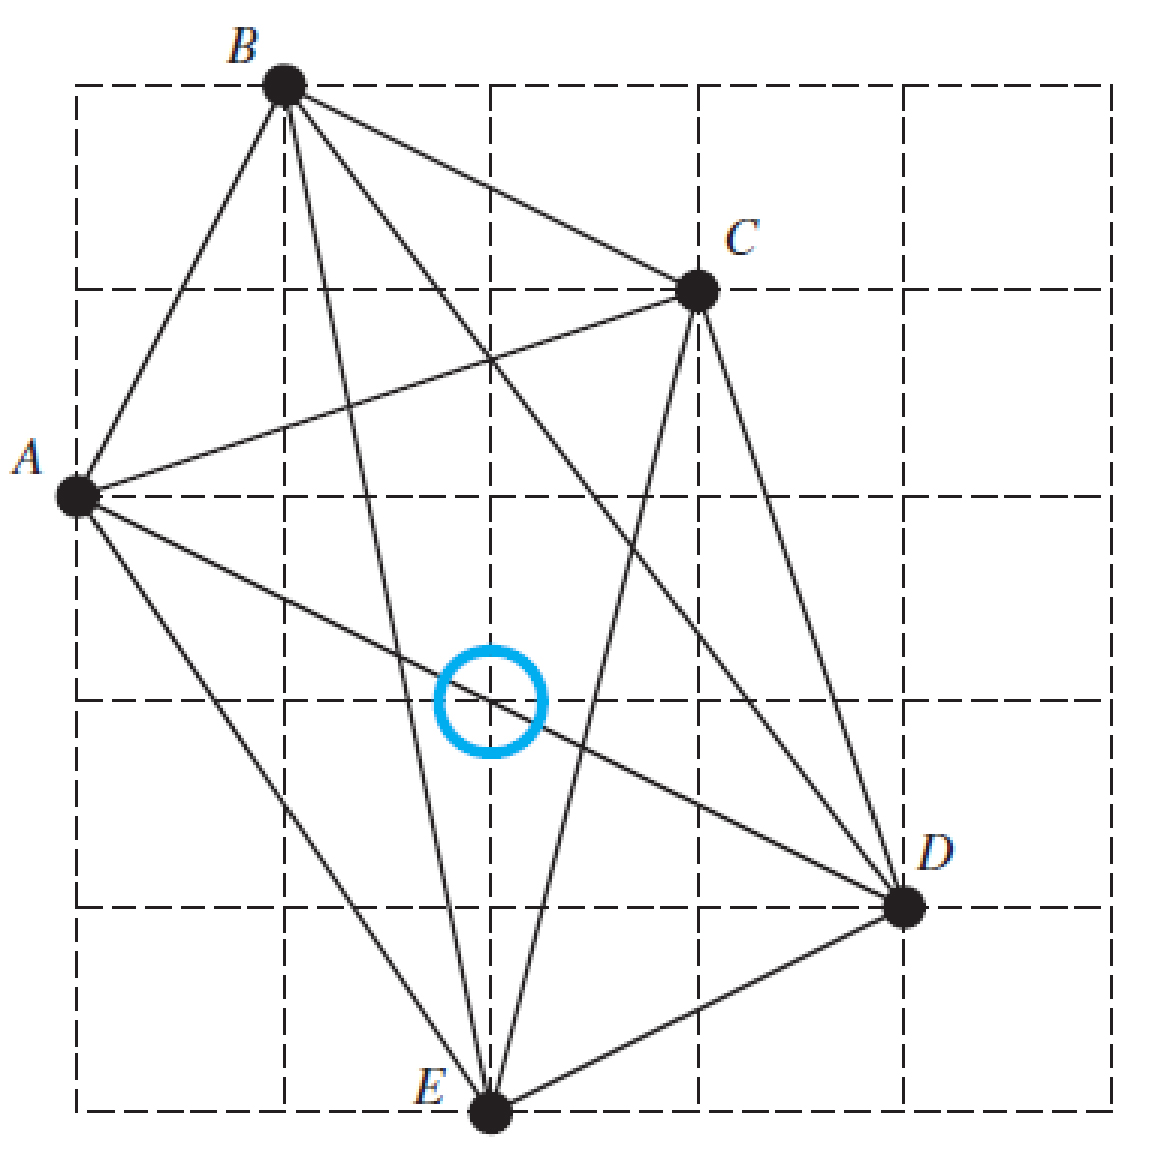
\includegraphics[scale=0.34]{LattPont.jpg}
\column{0.7\textwidth}
\bl[Proposition]{Given five distinct lattice points in the plane (points with integer coordinates), at least one of the line segments determined by these points has a lattice point as its midpoint}
\end{columns}

\only<2>{\bl[Recall:]{
If $(a,b)$ and $(c,d)$ are two points in the plane then the midpoint of the line segment connecting them is $(\frac{a+c}{2},\frac{b+d}{2})$.}}

\uncover<3->{
\begin{proof}
Each lattice point is one of the following type:
\[
(even,even)\qquad (even,odd)\qquad (odd,even)\qquad (odd,odd)
\]
Since we are given five lattice points, the pigeonhole principle implies that two of these points have to be of the same type, let's say $(a,b)$ and $(c,d)$. Then both $a+c$ and $b+d$ are even and therefore the midpoint $(\frac{a+c}{2},\frac{b+d}{2})$ of the connecting segment has integer coordinates.
\end{proof}
}
\end{frame}

\begin{frame}
\center Do Problem 3 on the worksheet.
\end{frame}

\section{Cantor's theorem}
\begin{frame}{Cardinality of infinite sets}
\bl[Definition]{Two infinite sets $A$ and $B$  have the same cardinality if there is a bijection $f:A\to B$.}
For example $f:\mathbb{N}\to\mathbb{Z}$, defined by
\[
f(n)=\left\{\begin{array}{cc}
-n/2&\textrm{if $n$ is even},\\
(n+1)/2&\textrm{if $n$ is odd}
\end{array}\right.
\]
\begin{center}
\begin{tabular}{|c||c|c|c|c|c|c|c|c|c|c|c|}
\hline
$n$&0&1&2&3&4&5&6&7&8&9&\dots\\
\hline
$f(n)$&0&1&-1&2&-2&3&-3&4&-4&5&\dots\\
\hline
\end{tabular}
\end{center}
\itemb
\item Every natural appears exactly once in the first row. (One-to-one)
\item Every integer appears exactly once in the second row. (Onto)
\iteme
Therefore $f$ is a bijection and $\mathbb{N}$ and $\mathbb{Z}$ has the same cardinality.
\end{frame}

\begin{frame}{Cantor's theorem}
\bl[]{\textbf{Q}: Is this true for all infinite sets? -> Nope}
\bl[Theorem(Cantor's theorem)]{Let $A$ be a set. If $f:A\to 2^{A}$, then $f$ is not onto.}

\begin{proof}
Let $A$ be a set and $f:A\to 2^A$. To show that $f$ is not onto, we have to find a $B\in 2^A$ for which $\cancel{\exists}a\in A$ with $f(a)=B$. Let\vspace{-0.3cm}
\[
B=\{x\in A:x\notin f(x)\}.
\]\vspace{-0.7cm}

FTSC, assume $\exists a\in A$ such that $f(a)=B$. Then either $a$ is in $B$ or not.
\itemb
\item If $a\in B$, then $a\notin f(a)$. But $f(a)=B$ implies $a\in f(a)$. $\Rightarrow\Leftarrow$.
\item If $a\notin B=f(a)$, then by definition, $a\in B$. $\Rightarrow\Leftarrow$.
\iteme
Therefore there is no such $a$ and $f$ is not onto.
\end{proof}
\end{frame}

\begin{frame}{A more intuitive reading}
$A$ is the set of people in a company (not excluding companies with inifnitely many employees, actually that is the interesting case)
\begin{itemize}
\item The company names each committee after one of the employees.
\item Let "Joe" be the name of the committee of the people who are not a member of the committee named after them.
\end{itemize}
\bl[]{Q:Is Joe a member of "Joe"?}

\begin{itemize}
\item If yes then no by definition.
\item If no then yes by definition.
\end{itemize}
Each case is a contradiction!



\end{frame}

\begin{frame}
\bl[Proposition]{$''|\mathbb{R}|>|\mathbb{N}|''$.}

\begin{proof}
Define the function $f:2^{\mathbb{N}}\to\mathbb{R}$ by
\[
f(A)=\sum_{a\in A}10^{-a}.
\]
In decimals, $f(A)$ is a number with ones exactly at every position corresponding to all $a\in A$. E.g.
\[
f(\{1,2,4\})=10^{-1}+10^{-2}+10^{-4}=0.1101
\]
Therefore if $A_1\neq A_2$, then $f(A_1)\neq f(A_2)$ and $f$ is one-to one. Therefore
\[
''|\mathbb{N}|<|2^{\mathbb{N}}|\leq|\mathbb{R}|''.\qedhere
\]
\end{proof}
\end{frame}

\end{document}